\documentclass[11pt,a4paper]{article}
\usepackage[margin=2cm]{geometry}
\usepackage{amsmath,amssymb}
\usepackage{xcolor}
\usepackage{enumitem}
\usepackage{tcolorbox}
\usepackage{listings}
\usepackage{hyperref}
\usepackage{array}
\usepackage{tikz}
\usetikzlibrary{positioning,arrows.meta,fit,calc}
\tcbuselibrary{breakable,skins}

\definecolor{kw}{HTML}{8B0058}
\definecolor{cmt}{HTML}{6A8F4B}
\definecolor{str}{HTML}{B36B00}
\definecolor{bg}{HTML}{FBFAF7}
\definecolor{hi}{HTML}{D63A6F}
\definecolor{accent}{HTML}{1F4E79}
\definecolor{warn}{HTML}{B91C1C}

\hypersetup{colorlinks=true,linkcolor=accent,urlcolor=accent}

\lstdefinelanguage{sv}{
  morekeywords={module,endmodule,input,output,logic,reg,wire,always,always_ff,always_comb,posedge,negedge,assign,if,else,begin,end,case,endcase,for,while,initial,parameter,localparam,typedef,struct,packed,union,enum,task,endtask,function,endfunction,return,break,continue,default,generate,endgenerate,genvar},
  morecomment=[l]//,
  morecomment=[s]{/*}{*/},
  morestring=[b]",
}

\lstdefinelanguage{asm}{
  morekeywords={add,addi,sub,lw,sw,beq,bne,bnez,beqz,jal,jalr,mv,li,mul,and,or,xor,lr,sc,call,ret,ecall,sret,fence,nop},
  morecomment=[l]\#,
  morestring=[b]",
}

\lstdefinestyle{c}{
  basicstyle=\ttfamily\footnotesize,
  keywordstyle=\color{kw}\bfseries,
  commentstyle=\color{cmt}\itshape,
  stringstyle=\color{str},
  backgroundcolor=\color{bg},
  frame=single,
  rulecolor=\color{black!20},
  framesep=4pt,
  numbers=none,
  showstringspaces=false,
  breaklines=true,
}
\lstset{style=c}

\newtcolorbox{must}{colback=hi!8,colframe=hi!75!black,boxrule=0.7pt,arc=2pt,
  fonttitle=\bfseries,title=Exam-critical,breakable}
\newtcolorbox{useful}{colback=accent!6,colframe=accent!60!black,boxrule=0.6pt,arc=2pt,
  fonttitle=\bfseries,title=Worth knowing,breakable}
\newtcolorbox{gotcha}{colback=warn!6,colframe=warn!70!black,boxrule=0.6pt,arc=2pt,
  fonttitle=\bfseries,title=Gotcha,breakable}
\newtcolorbox{plain}[1]{colback=gray!5,colframe=gray!50!black,boxrule=0.5pt,arc=2pt,
  fonttitle=\bfseries,title=#1,breakable}

\setlength{\parindent}{0pt}
\setlength{\parskip}{4pt}

\title{\vspace{-1.5cm}\textbf{Introduction to Computer Architecture} \\[2pt] \large The 80/20 Revision Guide}
\author{\small Part IB --- Cambridge CST}
\date{}

\begin{document}
\maketitle
\vspace{-0.8cm}

\section*{How this guide is organised}

The Computer Architecture paper (Paper 5) sets three questions per year. Across \textbf{four years of past papers (2022--2025, 12 questions)} --- the course is newer than most --- the topic distribution is:

\begin{center}
\begin{tabular}{lcc}
\hline
\textbf{Topic} & \textbf{Appearances} & \textbf{Share} \\
\hline
Cache design \& memory hierarchy        & 4 & 33\% \\
Multicore \& parallel processing (incl.\ coherence, sync) & 4 & 33\% \\
Pipelining \& hazards (incl.\ microarchitecture) & 4 & 33\% \\
SystemVerilog \& FPGA / digital design   & 4 & 33\% \\
RISC-V ISA \& load-store architecture    & 3 & 25\% \\
DRAM operations                          & 2 & 17\% \\
Virtual memory / memory protection       & 2 & 17\% \\
Branch and hazard handling               & 1 &  8\% \\
Exceptions \& coprocessors               & 1 &  8\% \\
Amdahl's law \& performance              & 1 &  8\% \\
Power efficiency \& dark silicon         & 1 &  8\% \\
Side-channel attacks / hardware security & 1 &  8\% \\
\hline
\end{tabular}
\end{center}

\textbf{80/20 verdict.} \textbf{Caches, pipelining, multicore (with cache coherence), and SystemVerilog account for roughly 80\% of marks.} The pattern of the paper is: question (a) is digital-design / SystemVerilog, question (b) is microarchitecture-flavoured (pipeline or cache), question (c) is the system-level paper-stretcher (multicore, virtual memory, security).

This document goes in that order: \textbf{must-know first, then important, then context}.

\hrulefill

\section{The Big Four (80\% of marks)}

\subsection{Caches and the memory hierarchy}

\begin{must}
This is the single most consistent question topic. Expect: ``calculate the miss rate / CPI / cache size for these parameters,'' ``compare direct-mapped, set-associative, fully-associative,'' ``explain write-through vs write-back,'' ``classify these misses as compulsory / capacity / conflict.''
\end{must}

\subsubsection*{Why a hierarchy?}

Physics: at 5\,GHz, light travels only 60\,mm in one clock cycle, and electrical signals on chip $<$20\,mm. A large memory cannot also be low-latency. Solution: layer fast-small over slow-big and let \textbf{locality} make up the difference.

\begin{itemize}[leftmargin=*,itemsep=1pt]
  \item \textbf{Temporal locality:} a word accessed now is likely to be accessed again soon (loops, repeated variables).
  \item \textbf{Spatial locality:} words near a recent access are likely to be accessed soon (sequential code, array walks).
\end{itemize}

Typical numbers to know:

\begin{center}
\begin{tabular}{lll}
\hline
Level & Latency & Size \\
\hline
L1 SRAM (on-chip)   & 1--9 cycles      & tens of KiB \\
L2 SRAM             & $\sim$20 cycles  & 256 KiB--1 MiB \\
L3 SRAM (LLC)       & $\sim$40 cycles  & MiBs--tens of MiB \\
DRAM (off-chip)     & $\sim$100 cycles & GiBs \\
Disk / SSD          & ms / $\mu$s      & TiBs \\
\hline
\end{tabular}
\end{center}

\subsubsection*{Cache anatomy and the address split}

A direct-mapped cache splits the address into three fields:

\begin{center}
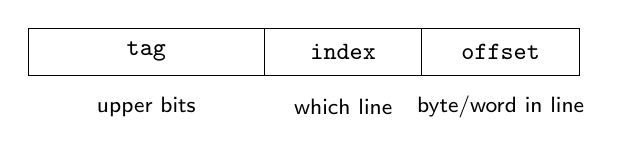
\begin{tikzpicture}[font=\small\ttfamily]
  \draw (0,0) rectangle (3,0.6) node[midway] {tag};
  \draw (3,0) rectangle (5,0.6) node[midway] {index};
  \draw (5,0) rectangle (7,0.6) node[midway] {offset};
  \node[font=\sffamily\footnotesize] at (1.5,-0.4) {upper bits};
  \node[font=\sffamily\footnotesize] at (4,-0.4) {which line};
  \node[font=\sffamily\footnotesize] at (6,-0.4) {byte/word in line};
\end{tikzpicture}
\end{center}

\textbf{Worked sizing example.} 32-bit address, 32\,KiB cache, 64-byte lines, direct-mapped.
\begin{itemize}[leftmargin=*,itemsep=1pt]
  \item \textbf{Offset:} $\log_2 64 = 6$ bits.
  \item \textbf{Number of lines:} $32 \text{ KiB} / 64 = 512$. \textbf{Index:} $\log_2 512 = 9$ bits.
  \item \textbf{Tag:} $32 - 9 - 6 = 17$ bits.
\end{itemize}

You will be asked this. Drill it.

\subsubsection*{Three placement policies}

\begin{itemize}[leftmargin=*,itemsep=1pt]
  \item \textbf{Direct-mapped:} each address maps to exactly one cache line. Cheap, fast, prone to conflict misses.
  \item \textbf{Fully associative:} an address can live anywhere; needs $N$ parallel tag comparators. Best hit rate, biggest hardware cost, scarcely used beyond TLBs and victim caches.
  \item \textbf{$N$-way set associative:} the common compromise. The cache is split into sets; each set has $N$ candidate slots; the index selects the set, then $N$ tag comparators check the set in parallel. Typical: 4--16 ways.
\end{itemize}

\subsubsection*{Write policies}

\begin{itemize}[leftmargin=*,itemsep=1pt]
  \item \textbf{Write-through:} write to cache and to next level. Always consistent; slow without a \textbf{write buffer} (which lets the core continue while writes drain).
  \item \textbf{Write-back:} write only to the cache; mark the line \textbf{dirty}. On eviction of a dirty line, write to next level. Faster on average, more complex.
  \item \textbf{Write-allocate} vs \textbf{write-around} on a write miss: do we fetch the line into cache, or write past it?
\end{itemize}
The common pairing: write-back + write-allocate. The other common pairing: write-through + no-allocate.

\subsubsection*{The three C's of misses}

\begin{itemize}[leftmargin=*,itemsep=1pt]
  \item \textbf{Compulsory (cold):} first access to a block. Reduced by larger lines / prefetching.
  \item \textbf{Capacity:} working set bigger than cache. Reduced by a bigger cache.
  \item \textbf{Conflict:} multiple addresses competing for the same set. Reduced by higher associativity. \emph{Wouldn't happen in a fully-associative cache.}
\end{itemize}

\subsubsection*{The standard CPI/AMAT calculation}

\begin{must}
This appears almost every year. Memorise the formulas.
\end{must}

\textbf{Average Memory Access Time:} $\text{AMAT} = t_{\text{hit}} + r_{\text{miss}} \cdot t_{\text{penalty}}$.

\textbf{Effective CPI (one cache):}
$$\text{CPI}_{\text{eff}} = \text{CPI}_{\text{base}} + r_{\text{miss/instr}} \cdot t_{\text{penalty (cycles)}}$$

\textbf{Worked example (Patterson \& Hennessy).} Base CPI = 1, clock = 4\,GHz, miss rate/instruction = 2\%, main memory access = 100\,ns.
\begin{itemize}[leftmargin=*,itemsep=1pt]
  \item Miss penalty = $100\,\text{ns} / 0.25\,\text{ns/cycle} = 400$ cycles.
  \item CPI = $1 + 0.02 \times 400 = 9$.
\end{itemize}
\textbf{Add an L2:} access time 5\,ns, global miss rate to DRAM = 0.5\%.
\begin{itemize}[leftmargin=*,itemsep=1pt]
  \item L1-miss-L2-hit penalty = 20 cycles. L1-miss-L2-miss extra penalty = 400.
  \item CPI = $1 + 0.02 \times 20 + 0.005 \times 400 = 3.4$. Speedup = $9 / 3.4 \approx 2.6$.
\end{itemize}

\subsubsection*{Cache design trade-off table (memorise)}

\begin{center}
\begin{tabular}{p{4.5cm}p{4.5cm}p{5.5cm}}
\hline
\textbf{Change} & \textbf{Effect on miss rate} & \textbf{Cost} \\
\hline
Larger cache       & Capacity misses $\downarrow$    & Access time $\uparrow$ \\
Higher associativity & Conflict misses $\downarrow$  & Access time $\uparrow$, hardware $\uparrow$ \\
Larger line size   & Compulsory misses $\downarrow$, then $\uparrow$ (pollution) & Miss penalty $\uparrow$ \\
Add a victim cache & Some conflict misses caught     & Tiny extra hardware \\
\hline
\end{tabular}
\end{center}

\subsection{Pipelining and hazards}

\begin{must}
Two question patterns: (i) ``draw a pipeline diagram for this code, mark stalls and forwarding paths''; (ii) ``compare branch prediction strategies''; (iii) ``calculate speedup of pipelined vs single-cycle.'' Always relative to the canonical \textbf{5-stage RISC-V pipeline.}
\end{must}

\subsubsection*{The 5 stages}

\begin{enumerate}[leftmargin=*,itemsep=0pt]
  \item \textbf{IF} --- instruction fetch from I-memory
  \item \textbf{ID} --- instruction decode, register file read
  \item \textbf{EX} --- ALU operation or address calculation
  \item \textbf{MEM} --- data memory access (load/store only)
  \item \textbf{WB} --- write result back to register file
\end{enumerate}

\textbf{Speedup intuition.} If all stages take the same time $T$, a non-pipelined cycle takes $5T$ but the pipelined throughput is one instruction per $T$. Maximum speedup = number of stages, in practice less due to stalls and unbalanced stages.

\subsubsection*{The three hazards}

\begin{itemize}[leftmargin=*,itemsep=1pt]
  \item \textbf{Structural} --- two instructions want the same resource at once. Cured by duplicating resources (separate I-cache and D-cache so IF and MEM don't fight for memory).
  \item \textbf{Data} --- an instruction needs the result of one still in flight.
  \item \textbf{Control} --- the next PC depends on a branch we haven't resolved yet.
\end{itemize}

\subsubsection*{Solving data hazards: forwarding (bypassing)}

The result of the EX stage is available at the end of EX, even though it hasn't been written back. \textbf{Forwarding} routes the EX output (or MEM output for loads) directly to the EX input of a following instruction.

\begin{center}
\begin{tabular}{ll}
\hline
Producer stage finishes at & Available to next-EX from \\
\hline
EX (ALU op)  & end of EX  $\Rightarrow$ next-cycle EX input \\
MEM (load)   & end of MEM $\Rightarrow$ \textbf{one bubble} before next EX \\
\hline
\end{tabular}
\end{center}

\textbf{Load-use hazard.} Even with full forwarding, you cannot forward from MEM to the immediately following EX (``forward backward in time''). You must stall one cycle, or reorder the code:

\begin{lstlisting}[language=asm]
# Original (causes one stall):
lw  x1, 0(sp)
lw  x2, 8(sp)
add x3, x1, x2   # uses x2 immediately - STALL
sw  x3, 24(sp)

# Reordered (no stall):
lw  x1, 0(sp)
lw  x2, 8(sp)
lw  x4, 16(sp)   # filler load
add x3, x1, x2
sw  x3, 24(sp)
\end{lstlisting}

\subsubsection*{Solving control hazards: prediction}

\textbf{Stall on branch} is correct but expensive --- one bubble per branch on a 5-stage pipeline, several on a deeper one.

\begin{itemize}[leftmargin=*,itemsep=1pt]
  \item \textbf{Static prediction:} ``backward branches taken, forward branches not taken'' --- exploits the fact that loop branches usually go back.
  \item \textbf{Dynamic prediction:} a branch predictor records the recent outcome (one-bit or two-bit saturating counter per branch entry). $\sim$95\% accuracy on real workloads.
  \item \textbf{On mispredict:} squash the in-flight wrong-path instructions and restart fetch from the correct PC.
\end{itemize}

\subsection{Multicore: coherence, consistency, synchronisation}

\begin{must}
The system-level question often lives here. You should be able to (a) walk the MSI/MESI protocol state machine for a specific sequence of reads and writes across cores, (b) explain why caches need a coherence protocol, (c) write a correct spin-lock using LR/SC, and (d) recognise when memory-ordering subtlety matters.
\end{must}

\subsubsection*{Cache coherence: the problem}

Multiple cores, private L1 caches, shared memory. If core 1 holds $X = 5$ in its L1 and core 2 writes $X = 7$, core 1's view becomes stale. Coherence makes the caches \textbf{behave as if there were a single shared memory.}

\textbf{Snoopy bus.} The cheap, classic mechanism: all caches sit on a broadcast bus and observe (\emph{snoop}) every other cache's transactions. Each cache line carries a \textbf{state} per coherence protocol.

\subsubsection*{MSI protocol}

Three states per line:

\begin{itemize}[leftmargin=*,itemsep=1pt]
  \item \textbf{M (Modified):} only this cache has it; value differs from memory. Implicit ``dirty.''
  \item \textbf{S (Shared):} this cache has a clean copy; other caches may too.
  \item \textbf{I (Invalid):} no valid copy here.
\end{itemize}

\textbf{Transitions (the most testable):}

\begin{center}
\begin{tabular}{p{4.5cm}p{1.7cm}p{8.5cm}}
\hline
\textbf{Action} & \textbf{From} & \textbf{To state \& effect} \\
\hline
Local read   & I & S; \texttt{BusRd}; if another cache has it in M, that cache writes back and goes to S \\
Local read   & S, M & same; no bus traffic \\
Local write  & I & M; \texttt{BusRdX} (read-with-intent-to-modify); other caches invalidate \\
Local write  & S & M; \texttt{Invalidate} broadcast; others go to I \\
Local write  & M & same; no bus traffic \\
Snoop \texttt{BusRd} of my M-line  & M & S; write back \\
Snoop \texttt{BusRdX}/Inv of my S or M & $\to$ & I \\
\hline
\end{tabular}
\end{center}

\textbf{MESI adds an \emph{Exclusive} state} for ``I have the only clean copy''; lets you go E$\rightarrow$M without bus traffic. \textbf{MOESI adds Owned} for shared-but-dirty (one cache holds the only up-to-date copy that others also share, replied to instead of memory).

\subsubsection*{Memory consistency}

Coherence settles \emph{when} writes to one location become visible. Consistency settles \emph{the order in which writes to different locations are observed.} Compilers and hardware reorder loads/stores --- the classic example:

\begin{lstlisting}[language=c]
// Initially A = B = 0
Core 1:                    Core 2:
A = 1;                     B = 1;
if (B == 0) X = 3;         if (A == 0) Y = 5;
\end{lstlisting}

Sequential-consistent answer: at most one of $X=3$ or $Y=5$ can hold. \textbf{In practice on modern relaxed memory models, both can happen} because the read of B (resp.\ A) can be reordered before the write. Cure: \textbf{memory fence} (\verb|fence rw,rw|) between the write and the read.

\subsubsection*{Atomic primitives: LR/SC on RISC-V}

\textbf{Load-Reserved / Store-Conditional} replaces test-and-set. The store-conditional succeeds only if no other write to the same line happened in the interval; otherwise the SC fails and you retry.

\begin{lstlisting}[language=asm]
# Efficient spin lock: read until it looks free, only then attempt SC
lock: lr.w   x4, (x1)        # load-reserved
      bne    x4, zero, lock  # is lock taken? spin (no writes!)
      li     x3, 1
      sc.w   x3, x3, (x1)    # store-conditional
      bne    x3, zero, lock  # SC failed - retry
      # ... critical section ...
unlock:
      sw     zero, 0(x1)
\end{lstlisting}

\textbf{Why the inner-loop read matters.} A naive ``test-and-set'' that writes every iteration thrashes the cache coherence protocol --- every core's spin pulls the lock cache line into M state, evicting it from everyone else. The version above only reads in the spin (line stays in S across all spinners), and only attempts the write when the lock looks free.

\subsection{Digital design: SystemVerilog \& FPGAs}

\begin{must}
The opening question on most papers. You will be asked to write or read SystemVerilog for a small synchronous circuit (a counter, a multiplexer, a small state machine, a piece of a datapath), and to reason about FPGA mapping (LUTs, flip-flops, block RAM, DSP).
\end{must}

\subsubsection*{Synchronous design fundamentals}

\begin{itemize}[leftmargin=*,itemsep=1pt]
  \item \textbf{Clocked elements} are D flip-flops; combinational logic between them computes the next state.
  \item \textbf{Setup time}: input D must be stable for $t_{\text{su}}$ \emph{before} the clock edge.
  \item \textbf{Hold time}: D must remain stable for $t_{\text{h}}$ \emph{after} the edge.
  \item \textbf{Critical path} = the longest combinational delay between any two registers. Sets the maximum clock frequency: $f_{\max} = 1/(t_{\text{cq}} + t_{\text{logic}} + t_{\text{su}})$.
\end{itemize}

\subsubsection*{SystemVerilog skeleton}

\begin{lstlisting}[language=sv]
module counter2bit(
    input  logic       clk,
    input  logic       rst_n,
    input  logic       go,
    output logic [1:0] n);

  always_ff @(posedge clk or negedge rst_n)
    if (!rst_n)   n <= 2'b00;
    else if (go)  n <= n + 2'b01;

endmodule
\end{lstlisting}

\textbf{The three \texttt{always} blocks to know:}
\begin{itemize}[leftmargin=*,itemsep=1pt]
  \item \verb|always_ff @(posedge clk)| --- synthesises to registers (flip-flops). Use \verb|<=| (non-blocking).
  \item \verb|always_comb| --- combinational logic. Use \verb|=| (blocking). Every output must be assigned on every path or you create unwanted latches.
  \item \verb|always_latch| --- explicit level-sensitive latch. Avoid except for tools that need it.
\end{itemize}

\textbf{Blocking vs non-blocking.} In \verb|always_ff|, \verb|a <= b; b <= a;| swaps both atomically (non-blocking: RHS evaluated first, LHS updated at clock edge). With \verb|a = b; b = a;| you'd just set both to the old $b$.

\subsubsection*{A small finite state machine}

\begin{lstlisting}[language=sv]
typedef enum logic [1:0] { IDLE, BUSY, DONE } state_t;
state_t state, next_state;

always_ff @(posedge clk or negedge rst_n)
    if (!rst_n) state <= IDLE;
    else        state <= next_state;

always_comb begin
    next_state = state;             // default to hold
    case (state)
        IDLE: if (start) next_state = BUSY;
        BUSY: if (done)  next_state = DONE;
        DONE:            next_state = IDLE;
    endcase
end
\end{lstlisting}

\textbf{The two-process FSM pattern}: one \verb|always_ff| for state register, one \verb|always_comb| for next-state and outputs. Easier to debug, no implicit latches.

\subsubsection*{FPGA resources}

An FPGA is roughly a sea of:
\begin{itemize}[leftmargin=*,itemsep=1pt]
  \item \textbf{LUTs} (Look-Up Tables) --- typically 4--6 input, each a tiny programmable truth table. Implement combinational logic.
  \item \textbf{Flip-flops} attached to LUTs --- state.
  \item \textbf{Block RAM (BRAM)} --- dedicated SRAM blocks, $\sim$kilobits each. Used for caches, FIFOs, register files.
  \item \textbf{DSP blocks} --- hard-wired multiply-accumulate units, for ML and signal processing.
  \item \textbf{Routing fabric} --- the programmable interconnect, where most of the area and delay live.
\end{itemize}

\textbf{Implication for caches:} a direct-mapped cache maps neatly onto BRAM (one read port, one write port, sequential). A fully-associative cache requires $N$ tag comparators in parallel --- on an FPGA those have to be built from registers + LUTs, blowing up area. \emph{This is the FPGA-specific reason set-associative is the common compromise.}

\hrulefill

\section{The Second Tier}

\subsection{RISC-V ISA basics}

\begin{useful}
You don't need to memorise every instruction. You do need: register conventions, the four instruction formats, the basic operations, and \textbf{the RISC philosophy} of orthogonal, fixed-length, load-store ISA.
\end{useful}

\subsubsection*{The RISC philosophy in three bullets}

\begin{itemize}[leftmargin=*,itemsep=1pt]
  \item \textbf{Load-store architecture.} Arithmetic operates only on registers; memory is touched only by \texttt{lw}/\texttt{sw}.
  \item \textbf{Fixed-length, regular encoding.} Easy fetch and decode in one cycle. RV32: every base instruction is 32 bits.
  \item \textbf{Few, orthogonal instructions.} All ALU ops take the same operand layout; registers are general-purpose.
\end{itemize}

\subsubsection*{Register file (RV32I)}

32 integer registers \verb|x0|--\verb|x31|. \verb|x0| is hard-wired to zero. The ABI assigns roles:

\begin{center}
\begin{tabular}{lll}
\hline
Reg & ABI & Role \\
\hline
\verb|x0|      & \verb|zero|  & constant 0 \\
\verb|x1|      & \verb|ra|    & return address (caller-saved) \\
\verb|x2|      & \verb|sp|    & stack pointer (callee-saved) \\
\verb|x5--x7|, \verb|x28--x31| & \verb|t0--t6| & temporaries (caller-saved) \\
\verb|x8|, \verb|x9|, \verb|x18--x27| & \verb|s0--s11| & saved (callee-saved) \\
\verb|x10--x17|              & \verb|a0--a7| & args / return values (caller-saved) \\
\hline
\end{tabular}
\end{center}

\subsubsection*{Common instructions}

\begin{lstlisting}[language=asm]
add  x3, x2, x1     # x3 = x2 + x1
addi x3, x3, 1      # x3 = x3 + 1
lw   x4, 0(x3)      # x4 = MEM[x3 + 0]
sw   x4, 8(x3)      # MEM[x3 + 8] = x4
beq  x4, x5, label  # if x4 == x5, branch to label
jal  ra, foo        # ra = PC+4; PC = foo (call)
jalr zero, ra, 0    # PC = ra  (return)
\end{lstlisting}

\subsubsection*{CISC vs RISC}

\begin{center}
\begin{tabular}{p{6cm}p{8.5cm}}
\hline
\textbf{RISC (RISC-V, ARM)} & \textbf{CISC (x86)} \\
\hline
Fixed-length instructions (32-bit) & Variable-length (1--17 bytes) \\
Load-store: only \texttt{lw}/\texttt{sw} touch memory & Many instructions can have memory operands \\
Few, orthogonal ops ($\sim$50 in base ISA) & Hundreds of instructions, many redundant \\
Easy to pipeline and decode in parallel & Hard --- modern x86 decodes to micro-ops internally \\
Dominant in mobile, embedded, accelerators & Dominant in PC \& server for backward compatibility \\
\hline
\end{tabular}
\end{center}

\subsection{Virtual memory}

\begin{useful}
Appears in 2022-5-8, 2024-5-8. Expect: ``explain TLB, page table walker, page fault handler''; ``compute the address translation from this multi-level page table.''
\end{useful}

\subsubsection*{The mapping}

The processor produces a \textbf{virtual address}; hardware translates to a \textbf{physical address}. Translation is at the granularity of a \textbf{page} (typically 4\,KiB) or a \textbf{superpage} (e.g.\ 4\,MiB).

\textbf{Address split} for a 4\,KiB page on a 32-bit virtual address: low 12 bits are the page offset (unchanged), high 20 bits are the virtual page number (VPN), translated to a physical page number (PPN).

\subsubsection*{Page table}

An array of \textbf{Page Table Entries (PTEs)}, indexed by VPN. Each PTE holds the PPN plus permission/status bits (\texttt{R}, \texttt{W}, \texttt{X}, \texttt{V}alid, \texttt{D}irty, \texttt{A}ccessed, \texttt{U}ser, \texttt{G}lobal).

A flat 32-bit / 4\,KiB scheme would need $2^{20} \times 4$\,B = 4\,MiB per process --- mostly empty. Solution: \textbf{multi-level page tables.} On RISC-V Sv32: the 20-bit VPN splits into two 10-bit pieces; the upper 10 indexes into a top-level table whose entries either point to a leaf page or to a second-level table. Each sub-table is one page.

\subsubsection*{TLB --- the cache of PTEs}

A translation per memory access would double DRAM bandwidth and add hundreds of cycles. The \textbf{TLB} caches recent PTEs (16--512 entries, fully or highly associative). Typical: 1\,cycle hit, 10--100 cycles miss.

\textbf{TLB miss.} Either (a) hardware page-table walker reads memory, fills the TLB, retries; or (b) raise a software exception and let the OS do it (older designs). Modern CPUs use hardware walkers.

\textbf{Page fault.} If the PTE says ``not present,'' the OS handles it: locate the page on disk, possibly evict a dirty page (write-back!), read in, update the PTE, restart the faulting instruction. Can cost \emph{millions} of cycles.

\subsubsection*{Memory protection}

The OS gives each process its own page table. On context switch, change the page-table base register (\verb|satp| on RISC-V). The \textbf{ASID} (address-space ID) is also held in TLB entries so a context switch doesn't have to flush the whole TLB. The OS lives in \textbf{Supervisor mode}; user processes in \textbf{User mode}; privileged instructions and registers (\verb|satp|, \verb|mtvec|, \verb|sepc|) are accessible only from privileged modes.

\subsection{Exceptions and interrupts}

\begin{useful}
Specifically tested in 2025-5-7. Be able to distinguish exception (synchronous, instruction-caused), interrupt (asynchronous, external) and software exception (\texttt{ecall}).
\end{useful}

\begin{itemize}[leftmargin=*,itemsep=1pt]
  \item \textbf{Exceptions} are synchronous to the instruction stream: divide-by-zero, illegal instruction, page fault, misaligned access.
  \item \textbf{Interrupts} are asynchronous: timer, DMA-complete, I/O device. The current instruction completes; the handler runs.
  \item \textbf{Software exceptions} (\verb|ecall|, \verb|ebreak|) are deliberate transitions into a more privileged mode --- system calls.
\end{itemize}

\textbf{RISC-V mechanism.} On any trap: save current PC to \verb|sepc| (or \verb|mepc|), put cause in \verb|scause|, jump to handler at \verb|stvec|. Handler completes; \verb|sret| restores PC and privilege.

\subsection{Amdahl's and Gustafson's laws}

\begin{useful}
Tested in 2023-5-7. One-formula questions; learn the formulas and a sentence on each.
\end{useful}

\textbf{Amdahl} (fixed problem, scale cores). For sequential fraction $B$ and $n$ cores:
$$\text{Speedup}(n) = \frac{1}{B + (1 - B)/n}$$
\textbf{Implication.} As $n \to \infty$, $\text{Speedup} \to 1/B$. If 10\% is sequential, you cap at 10$\times$ speedup, no matter how many cores. \emph{The sequential bottleneck dominates.}

\textbf{Gustafson} (fixed time, scale problem). $\text{Speedup}(n) = n - (n-1)B$. The optimistic counterpart: with more cores you tackle bigger problems, and the parallel fraction grows.

\textbf{When examiners ask you to ``critique'':} Amdahl assumes the problem is fixed; Gustafson assumes time is fixed. Real workloads sit between these two extremes.

\hrulefill

\section{The Third Tier (context \& flavour)}

\subsection{The eight great ideas in computer architecture}

A useful mnemonic for ``what is computer architecture about'' --- comes straight from Patterson \& Hennessy:

\begin{enumerate}[leftmargin=*,itemsep=1pt]
  \item Design for Moore's law (assume next year's chip has $\sim$2$\times$ transistors).
  \item Use abstraction to simplify design (HLL $\rightarrow$ assembly $\rightarrow$ machine code).
  \item Make the common case fast.
  \item Performance via parallelism (ILP, DLP, TLP).
  \item Performance via pipelining (one production line per stage).
  \item Performance via prediction (branch, cache, value).
  \item Hierarchy of memories (caches).
  \item Dependability via redundancy (ECC, RAID, lockstep cores).
\end{enumerate}

\subsection{Performance equation}

$$\text{CPU time} = \frac{\text{instructions}}{\text{program}} \times \frac{\text{cycles}}{\text{instruction}} \times \frac{\text{seconds}}{\text{cycle}}$$

\textbf{What changes what:}

\begin{center}
\begin{tabular}{lccc}
\hline
\textbf{Affects} & \textbf{Instr count} & \textbf{CPI} & \textbf{Clock period} \\
\hline
Program             & $\bullet$ & $\bullet$ & \\
Compiler            & $\bullet$ & $\bullet$ & \\
ISA                 & $\bullet$ & $\bullet$ & $\bullet$ \\
Microarchitecture   &           & $\bullet$ & $\bullet$ \\
Implementation tech &           &           & $\bullet$ \\
\hline
\end{tabular}
\end{center}

\subsection{DRAM operation (one-paragraph version)}

A DRAM chip is a 2D array of bit-cells, each a single capacitor. An access:
\begin{enumerate}[leftmargin=*,itemsep=1pt]
  \item \textbf{Row activate} (RAS): the row address is decoded; the entire row is pulled into a row buffer, destroying the row's contents in the array.
  \item \textbf{Column access} (CAS): one or more columns are read from the row buffer.
  \item \textbf{Precharge}: the row buffer is written back to the array, restoring it.
\end{enumerate}
This is why DRAM is \textbf{burst-oriented} (read many words from one activated row, cheap) and \textbf{row-locality-sensitive} (different row $\Rightarrow$ full activate/precharge cycle, expensive). DDR4 typically does 8 bursts of 64 bits = 64\,B per transfer --- not coincidentally, the standard cache line size.

\textbf{DRAM cells must be refreshed} (typically every $\sim$64\,ms) because charges leak. The refresh controller schedules these without disrupting normal access.

\subsection{Flynn's taxonomy}

\begin{center}
\begin{tabular}{lll}
\hline
& \textbf{Single instr} & \textbf{Multi instr} \\
\hline
\textbf{Single data}  & SISD (classic CPU) & MISD (rare; redundancy) \\
\textbf{Multi data}   & SIMD (vectors, GPUs) & MIMD (multicore) \\
\hline
\end{tabular}
\end{center}

\textbf{Note SIMT} (Single Instruction, Multiple Thread, used by GPUs) is essentially SIMD with the appearance of independent threads; the hardware groups threads into \textbf{warps} and executes them in lockstep.

\subsection{Dark silicon and the energy wall}

Transistors keep shrinking, but \textbf{Dennard scaling} (voltage scaling with size) ended around 2005. Today you can fit more transistors on a chip than you can power simultaneously --- the unpowered ones are \textbf{dark silicon}. Consequence: clock speeds plateaued; instead, vendors added more cores and \textbf{accelerators} (TPU, GPU, NIC offload, crypto engines, codecs). Energy efficiency, not transistor count, is now the limiter.

\subsection{Side-channel attacks (Spectre)}

\begin{useful}
Specifically tested in 2025-5-8. Be able to explain the mechanism in 3 sentences.
\end{useful}

\textbf{Mechanism.} Speculative execution lets a CPU run instructions past a branch before knowing whether the branch is taken. If the branch turns out mispredicted, those instructions are squashed --- \emph{architecturally}. But they still left side effects in the \textbf{cache}. By timing subsequent loads, an attacker can tell which addresses were touched, leaking secret-dependent information.

\textbf{Spectre example sketch:}
\begin{lstlisting}[language=c]
uint8_t A[10], B[256 * 64];
void victim(size_t i) {
    if (i < 10) {                  // mispredicted as taken
        uint8_t v = A[i];           // out-of-bounds read; speculative
        uint8_t junk = B[64 * v];   // touches a cache line indexed by secret
    }
}
// Attacker times reads of B and infers v from which line is now warm.
\end{lstlisting}

\textbf{Mitigations.} Speculation barriers (\verb|lfence|), retpolines, hiding speculative cache state (InvisiSpec), and tracking taint (STT). All have a performance cost.

\hrulefill

\section{The one-page exam checklist}

\begin{must}
If you have one hour to revise, do these in order:
\begin{enumerate}[leftmargin=*,itemsep=2pt]
  \item Be able to compute tag/index/offset bit widths from cache size, associativity, line size, address width.
  \item Be able to compute AMAT and effective CPI given miss rates and penalties --- one cache level and two.
  \item Be able to classify a sequence of accesses into compulsory / capacity / conflict misses.
  \item Be able to explain write-through vs write-back, write-allocate vs no-allocate, and the rationale for the common pairings.
  \item Be able to draw the 5-stage RISC-V pipeline, identify a data hazard in given assembly, and show where forwarding paths go.
  \item Be able to detect a load-use hazard and either insert a stall bubble or reorder code to remove it.
  \item Be able to walk MSI (or MESI) through a worked sequence of reads/writes across two cores.
  \item Be able to write a correct LR/SC spin-lock and explain why naive test-and-set thrashes coherence.
  \item Be able to write a small SystemVerilog FSM (two-process pattern) without creating implicit latches.
  \item Know which FPGA resource maps to what: LUT $\rightarrow$ combinational, FF $\rightarrow$ state, BRAM $\rightarrow$ cache/FIFO, DSP $\rightarrow$ MAC.
  \item Be able to walk a multi-level page table translation and explain TLB hits, TLB misses, page faults.
  \item Be able to state Amdahl's law, derive the asymptotic speedup, and contrast with Gustafson.
  \item Be able to explain Spectre in three sentences (speculative execution + cache side channel + timing).
\end{enumerate}
\end{must}

\vspace{0.4cm}
\begin{center}
\textit{Good luck.}
\end{center}

\end{document}
